In this section, we show empirical results of our algorithm on different transferring situations on two image benchmark datasets: MNIST\footnote{http://yann.lecun.com/exdb/mnist/} \cite{lampert2009learning} and USPS\footnote{http://www.cs.nyu.edu/~roweis/data.html}. We test the performance of our algorithm in different scenarios and show that SMTLe can outperform the other baseline transfer methods when the source and target domains are related and alleviate negative transfer while other baseline methods suffer.
\subsection{Dataset}
The MNIST database \cite{lecun1998gradient} (Mixed National Institute of Standards and Technology database) is a large database of handwritten digits that is commonly used for training various image processing systems. The database is also widely used for training and testing in the field of machine learning. It was created by "re-mixing" the samples from NIST's original datasets. The creators felt that since NIST's training dataset was taken from American Census Bureau employees, while the testing dataset was taken from American high school students, NIST's complete dataset was too hard. Furthermore, the black and white images from NIST were normalized to fit into a 28x28 pixel bounding box and anti-aliased, which introduced grayscale levels. In our experiment, we use a sub-set of MNIST dataset, containing 6,000 examples for 10 classes (from digit 0 to 9). We also use another handwritten digital dataset USPS \cite{hull1994database}. USPS contains 11,000 images and the data is evenly distributed among 10 classes, i.e. 1,100 examples for each digit. Each digit is represented as a 16x16 greyscale image.
 
For each of the datasets, we randomly split them into 3 sets: the large source dataset (100 examples per class for both dataset) to train the source models, the small target training set (5/10/15/20/25 examples per class for both datasets) to train target model and the large target testset (4700 and 9700 examples for MNIST and USPS respectively) to evaluate the performance of the target model.

\subsection{Baseline methods and experiment setup}
We compare our algorithm with two kinds of baselines. The first one is methods without leveraging any prior knowledge (no transfer baselines). The second consists of some methods with transfer techniques. 

We select 2 no transfer baselines:
\textbf{No transfer (NT):} LS-SVM trained only on target data. Any transfer algorithm that performs worse than it suffers from negative transfer. \textbf{Batch:} We combined the source and target data, assuming that we have full access to all data, to train the LS-SVM. The result of this baseline might be considered as the best performance achieved when no noise is added to the source data.


We select the 3 HTL baseline methods, \textbf{MKTL \cite{jie2011multiclass}}, \textbf{Multi-KT \cite{tommasi2014learning}}, \textbf{PMT-SVM} \cite{aytar2011tabula} as our transfer baselines. In Multi-KT, there are 3 different strategies, Weighted Multi-KT, Single-KT and Average-KT. We use all the 3 strategies in our experiments and denote them as MKT\_m, MKT\_s and MKT\_a respectively. For PMT-SVM, we use grid search on $\{0.1,0.2,...,1\}$ for the weights of its projection matrix and report the best performance.
Also, we include the method (Feature+) discussed in Section \ref{sec:prob} which solve the hyperplane $\hat{w}$ directly. 
For our method SMTLe, we implement 2 adaptation strategies single-adaptation (SMTLe\_s) and multi-adaptation (SMTLe\_m). For SMTLe\_s, we choose the model that distinguishes the corresponding class in the source, i.e. choose the model to distinguish the class digit 1 in the source as the single source model for target binary model of the class digit 1. For SMTLe\_m, we choose all the source models for each target binary model.

%\textbf{MKTL \cite{jie2011multiclass}:} This method uses the output of source models as extra feature inputs and automatically determine from which source models to transfer and how much to transfer.


%\textbf{MULTI-KT \cite{tommasi2014learning}:} This method has similar idea with MKTL. It uses LOO error to determine how much to transfer from source models and convert it into solving the convex optimization problem.

%\textbf{MULTIpLE \cite{kuzborskij2013n}:} The basic setting of this method is similar to ours. It is designed to balance the performance between learning the new category and preserving the model from prior knowledge.

For all the experiments in this section, we adopt the same strategy as \cite{kuzborskij2013n} and \cite{tommasi2014learning}, using kernel averaging \cite{gehler2009feature} to compute the average of RBF kernels on RBF hyperparameter $\{2^{-5},2^{-4},...,2^8\}$. The penalty parameter $C$ is tuned via cross-validation on $\{10^{-5},10^{-4},...,10^8\}$ and the optimal value is reused for all the algorithms.
The transfer regularization parameter $\lambda$ in SMTLe is also set via cross-validation on $\{10^{-3},10^{-2},...,10\}$ respectively.

To generate difference source models with different relatedness to the target domain. We add the different level of the noise to the source training data and train the source models from the noisy source data. When there is no noise added to the source data, the source and target domain are identical (strongly related). As we add more noise, the distribution of the data in source and target domain become more different, i.e. the source and target domain become less related (see Figure \ref{fig:noise}).

\begin{figure}
\centering
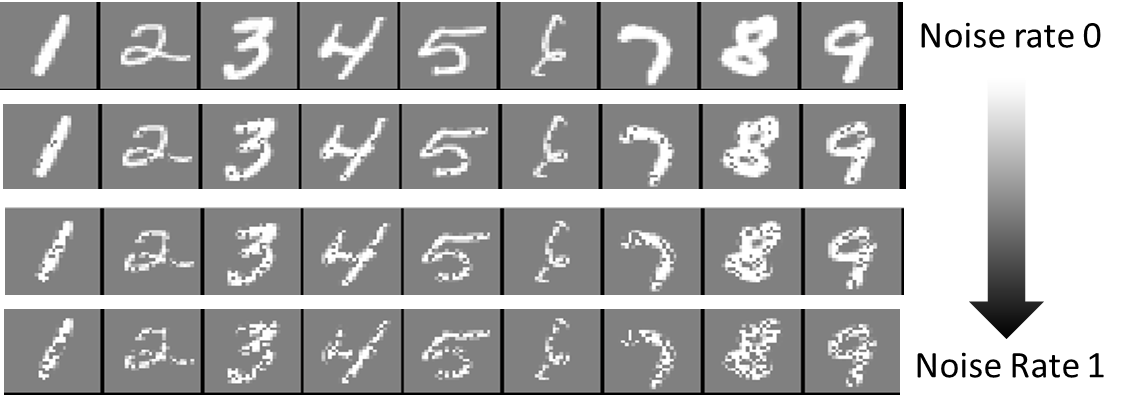
\includegraphics[scale=0.45]{fig/noise.png}
\caption{We add the noise to the source data to generate the source domain with different relatedness to the target domain. From the images we  can see that the source domain is still related to the target domain in different level of the noise rate}\label{fig:noise}
\end{figure}

\subsection{Experiment result \& analysis}
\begin{table*}[htbp]
   \subfloat[Results on MNIST]{\resizebox{0.5\textwidth}{!}{
    \begin{tabular}{|c|c|c|c|c|c|c|c|}
     \hline 
      & \multicolumn{7}{c|}{Noise Level} \\ \hline
     & 0.0 & 0.2 & 0.3 & 0.5 & 0.8 & 0.9 & 1.0\\ \hline
      SMTLe\_s & \textbf{87.23} & \textbf{86.40} & \textbf{85.81} & \textbf{84.63} & \textbf{81.51} & \textbf{79.67} & \textbf{78.10}\\ 
      SMTLe\_m & 82.94 & 80.20 & 79.05 & 76.56 & 72.10 & 69.57 & 68.09\\ 
      MKT\_{m} & 61.96* & 57.14* & 55.18* & 50.67* & 45.16* & 43.72* & 42.73*\\ 
      MKT\_{s} & 86.63 & 82.33 & 79.78 & 74.61 & 67.51 & 65.52 & 64.06\\ 
      MKT\_{a} & 62.94 & 63.04 & 63.03 & 62.91 & 62.93 & 62.98 & 62.89\\ 
      MKTL & 70.06 & 55.63* & 60.42* & 41.57* & 40.44* & 42.22* & 31.44*\\ 
      PMT & 63.54 & 63.54 & 63.54 & 63.54 & 63.54 & 63.54 & 63.54\\ 
      Feature+ & 66.99 & 61.72* & 59.13* & 54.27* & 46.46* & 44.44* & 42.67*\\ 
      NT & 62.87 & 62.87 & 62.87 & 62.87 & 62.87 & 62.87 & 62.87\\ 
      Batch & 87.39 & 84.42 & 82.40 & 76.83 & 62.86* & 57.33* & 51.16*\\ 
\hline\end{tabular}}}%{body}
\subfloat[Results on USPS]{
    \resizebox{0.5\textwidth}{!}{
     \begin{tabular}{|c|c|c|c|c|c|c|c|}
          \hline 
          & \multicolumn{7}{c|}{Noise Level} \\ \hline
          & 0.0 & 0.2 & 0.3 & 0.5 & 0.8 & 0.9 & 1.0\\ \hline
           SMTLe\_s & \textbf{91.12} & 89.79 & 89.23 & 88.06 & 86.22 & 85.33 & 84.60\\ 
           SMTLe\_m & 90.78 & \textbf{89.85} & \textbf{89.42} & \textbf{88.55} & \textbf{86.80} & \textbf{85.96} & \textbf{84.91}\\ 
           MKT\_{m} & 86.80 & 84.80 & 83.57 & 81.02 & 75.96 & 74.53* & 72.73*\\ 
           MKT\_{s} & 64.18* & 61.39* & 61.80* & 62.93* & 64.85* & 65.29* & 65.55*\\ 
           MKT\_{a} & 75.76 & 75.76 & 75.75 & 75.79 & 75.75 & 75.78 & 75.84\\ 
           MKTL & 90.24 & 88.13 & 86.20 & 86.07 & 81.82 & 80.18 & 80.14\\ 
           PMT & 75.89 & 75.89 & 75.9 & 75.88 & 75.88 & 75.88 & 75.87\\ 
           Feature+ & 88.42 & 86.56 & 85.28 & 83.23 & 79.79 & 78.68 & 77.17\\ 
           NT & 75.75 & 75.75 & 75.75 & 75.75 & 75.75 & 75.75 & 75.75\\ 
           Batch & 91.65 & 90.38 & 89.58 & 87.36 & 82.55 & 80.52 & 77.84\\ 
     \hline\end{tabular}}}%
     \caption{Experiment results on 5 examples per class in target training set. We show the percentage of accuracy across the 10 classes on different noise level. We use "*" to denote the results suffer from negative transfer}\label{tab:rs}
  \end{table*}%
  
We perform the algorithms on different scenarios where the different level of noise is added to the source data to train the source models. Still we use LS-SVM to train the source models. For each dataset, we use the accuracy across the 10 classes as the criterion to evaluate the performance of the algorithms. We randomly split the original datasets into 3 sets and run 10 times to report the average performance. 

We show the performance of different algorithms on the two datasets under different noise level in Table \ref{tab:rs}. We show more results with different size of training examples in the target set in Table \ref{tab:mnist} and Table \ref{tab:usps}. From Table \ref{tab:rs} we can see that when there is no noise in the source data, most transfer algorithms can leverage the knowledge of the source model. Our methods $SMTLe_s$ and $SMTLe_m$ achieve the best performance among all transfer methods, but still a slightly underperform the Batch method which can access all the data from both source and target training data. It is worthy to notice that the $MKT_m$ in MNIST and $MKT_s$ in USPS suffer from negative transfer even though there is no noise in the source data. This may cause by their weak regularization term which limits the transfer parameters within the ball with radium 1 (its default setting). The results could be improved if a better regularization can be found. As we add more noise into the source data, some of the transfer algorithms start to suffer from negative transfer. It is not surprising that all the methods (except for NT as no source knowledge is used) get a decreased performance. However, our methods can still outperform the other methods. In our method, the optimal transfer parameters can both limit the VC dimension and reduce empirical risk at the same time. This promise that the target model can still perform well on the unseen data even though the source models become less related to the target domain. We can also see that there are just 3 methods that don't suffer from negative transfer in both datasets, i.e. $SMTLe_s$,$SMTLe_m$ and $MKT_a$. However, we can see that $MKT_a$ is a more conservative method which is reluctant to leveraging the knowledge from the source model and as a result, it can successfully alleviate negative transfer and unable to fully exploit the knowledge from the source as well.

In summary, in this section, we empirically evaluate the performance of our method in different scenarios where there is different relatedness between the source and target domains. Comparing with some baseline methods we can see that our method can effectively leverage the knowledge from the source models and alleviate negative transfer when other baseline methods suffer.

\begin{table*}[h]
\subfloat[10 examples per class]
{\resizebox{0.5\textwidth}{!}{\begin{tabular}{|c|c|c|c|c|c|c|c|}
     \hline 
     & \multicolumn{7}{c|}{Noise Level} \\ \hline
     & 0.0 & 0.2 & 0.3 & 0.5 & 0.8 & 0.9 & 1.0\\ \hline
      SMTLe\_s & \textbf{88.13} & \textbf{86.98} & \textbf{86.62} & \textbf{85.44} & \textbf{84.26} & \textbf{83.61} & \textbf{82.79}\\ 
      SMTLe\_m & 87.29 & 85.20 & 83.81 & 81.47 & 77.74 & 76.45 & 76.26\\ 
      MKT\_{m} & 65.01* & 61.51* & 59.02* & 53.92* & 49.24* & 48.34* & 47.51*\\ 
      MKT\_{s} & 87.82 & 85.88 & 84.00 & 80.85 & 75.87 & 73.81 & 72.30\\ 
      MKT\_{a} & 72.37 & 72.32 & 72.36 & 72.30 & 72.32 & 72.32 & 72.25\\ 
      MKTL & 79.63 & 68.80* & 69.55* & 59.74* & 52.04* & 50.47* & 42.47*\\ 
      Feature+ & 77.60 & 73.33 & 70.73* & 64.90* & 56.86* & 54.40* & 52.3*\\ 
      PMT & 72.86 & 72.87 & 72.87 & 72.87 & 72.86 & 72.86 & 72.87\\ 
      NT & 72.22 & 72.23 & 72.23 & 72.23 & 72.23 & 72.23 & 72.23\\ 
      Batch & 87.46 & 84.78 & 82.96 & 78.04 & 65.96* & 60.97* & 55.65*\\ 
\hline\end{tabular}}}\qquad
\subfloat[15 examples per class]{\resizebox{0.5\textwidth}{!}{\begin{tabular}{|c|c|c|c|c|c|c|c|}
     \hline 
     & \multicolumn{7}{c|}{Noise Level} \\ \hline
     & 0.0 & 0.2 & 0.3 & 0.5 & 0.8 & 0.9 & 1.0\\ \hline
      SMTLe\_s & 88.63 & \textbf{87.52} & \textbf{87.12} & \textbf{86.33} & \textbf{85.57} & \textbf{85.04} & \textbf{84.65}\\ 
      SMTLe\_m & \textbf{88.92} & 86.98 & 85.99 & 84.01 & 80.69 & 80.08 & 79.28\\ 
      MKT\_{m} & 67.03* & 63.34* & 61.31* & 56.26* & 51.76* & 50.72* & 49.69*\\ 
      MKT\_{s} & 88.08 & 86.31 & 85.40 & 83.38 & 79.52 & 77.83 & 77.04\\ 
      MKT\_{a} & 76.19 & 76.16 & 76.19 & 76.12 & 76.14 & 76.16 & 76.11\\ 
      MKTL & 83.75 & 74.27* & 77.46 & 66.39* & 61.57* & 60.0* & 55.28*\\ 
      Feature+ & 81.87 & 78.54 & 76.63 & 72.25* & 64.45* & 61.88* & 59.67*\\ 
      PMT & 76.78 & 76.78 & 76.78 & 76.79 & 76.78 & 76.78 & 76.78\\ 
      NT & 76.09 & 76.10 & 76.10 & 76.10 & 76.10 & 76.10 & 76.10\\ 
      Batch & 87.72 & 85.20 & 83.57 & 79.29 & 68.95* & 64.36* & 59.8*\\ 
\hline\end{tabular}}}\\
\subfloat[20 examples per class]{\resizebox{0.5\textwidth}{!}{\begin{tabular}{|c|c|c|c|c|c|c|c|}
     \hline 
     & \multicolumn{7}{c|}{Noise Level} \\ \hline
     & 0.0 & 0.2 & 0.3 & 0.5 & 0.8 & 0.9 & 1.0\\ \hline
      SMTLe\_s & 88.87 & 87.81 & \textbf{87.28} & \textbf{86.50} & \textbf{85.98} & \textbf{85.64} & \textbf{85.27}\\ 
      SMTLe\_m & \textbf{89.39} & \textbf{87.97} & 87.06 & 85.47 & 82.63 & 81.95 & 81.32\\ 
      MKT\_{m} & 68.03* & 64.37* & 62.7* & 58.98* & 54.41* & 53.52* & 52.93*\\ 
      MKT\_{s} & 88.04 & 86.42 & 85.58 & 83.69 & 81.29 & 80.66 & 79.56\\ 
      MKT\_{a} & 78.68 & 78.64 & 78.65 & 78.62 & 78.63 & 78.63 & 78.60\\ 
      MKTL & 86.75 & 81.14 & 82.46 & 72.57* & 65.4* & 69.53* & 61.56*\\ 
      Feature+ & 83.80 & 80.99 & 79.29 & 75.54* & 68.46* & 66.12* & 63.97*\\ 
      PMT & 78.43* & 78.43* & 78.44* & 78.44* & 78.43* & 78.43* & 78.43*\\ 
      NT & 78.58 & 78.59 & 78.59 & 78.60 & 78.60 & 78.59 & 78.60\\ 
      Batch & 87.80 & 85.41 & 83.89 & 80.10 & 71.22* & 67.35* & 63.28*\\ 
\hline\end{tabular}}}\qquad
\subfloat[25 examples per class]{\resizebox{0.5\textwidth}{!}{\begin{tabular}{|c|c|c|c|c|c|c|c|}
     \hline 
     & \multicolumn{7}{c|}{Noise Level} \\ \hline
     & 0.0 & 0.2 & 0.3 & 0.5 & 0.8 & 0.9 & 1.0\\ \hline
      SMTLe\_s & 89.22 & 88.16 & 87.67 & \textbf{86.94} & \textbf{86.46} & \textbf{86.26} & \textbf{85.95}\\ 
      SMTLe\_m & \textbf{89.69} & \textbf{88.7} & \textbf{87.72} & 86.33 & 83.95 & 83.23 & 82.73\\ 
      MKT\_{m} & 69.15* & 66.04* & 64.23* & 60.71* & 56.0* & 54.9* & 54.53*\\ 
      MKT\_{s} & 88.21 & 86.6 & 85.87 & 84.14 & 82.02 & 81.51 & 81.04\\ 
      MKT\_{a} & 80.35 & 80.33 & 80.36 & 80.33 & 80.33 & 80.33 & 80.31\\ 
      MKTL & 87.50 & 84.39 & 81.88 & 72.97* & 70.57* & 70.17* & 62.88*\\ 
      Feature+ & 85.23 & 82.76 & 81.21 & 77.66* & 71.59* & 69.39* & 67.48*\\ 
      PMT & 79.58* & 79.59* & 79.59* & 79.59* & 79.59* & 79.59* & 79.58*\\ 
      NT & 80.27 & 80.29 & 80.28 & 80.29 & 80.29 & 80.29 & 80.29\\ 
      Batch & 88.02 & 85.80 & 84.33 & 80.92 & 73.36* & 69.99* & 66.27*\\ 
\hline\end{tabular}}}\caption{Results on MNIST with 10/15/20/25 positive examples for each class}\label{tab:mnist}
\end{table*}



\begin{table*}
\subfloat[10 examples per class]{\resizebox{0.5\textwidth}{!}{\begin{tabular}{|c|c|c|c|c|c|c|c|}
     \hline 
     & \multicolumn{7}{c|}{Noise Level} \\ \hline
     & 0.0 & 0.2 & 0.3 & 0.5 & 0.8 & 0.9 & 1.0\\ \hline
      SMTLe\_s & \textbf{91.12} & 89.79 & 89.23 & 88.06 & 86.22 & 85.33 & 84.60\\ 
      SMTLe\_m & 90.78 & \textbf{89.85} & \textbf{89.42} & \textbf{88.55} & \textbf{86.80} & \textbf{85.96} & \textbf{84.91}\\ 
      MKT\_{m} & 86.80 & 84.80 & 83.57 & 81.02 & 75.96 & 74.53* & 72.73*\\ 
      MKT\_{s} & 64.18* & 61.39* & 61.80* & 62.93* & 64.85* & 65.29* & 65.55*\\ 
      MKT\_{a} & 75.76 & 75.76 & 75.75 & 75.79 & 75.75* & 75.78 & 75.84\\ 
      MKTL & 90.24 & 88.13 & 86.20 & 86.07 & 81.82 & 80.18 & 80.14\\ 
      Feature+ & 88.42 & 86.56 & 85.28 & 83.23 & 79.79 & 78.68 & 77.17\\ 
      PMT & 75.89 & 75.89 & 75.90 & 75.88 & 75.88 & 75.88 & 75.87\\ 
      NT & 75.75 & 75.75 & 75.74 & 75.76 & 75.76 & 75.76 & 75.74\\ 
      Batch & 91.65 & 90.38 & 89.58 & 87.36 & 82.55 & 80.52 & 77.84\\ 
\hline\end{tabular}}} \qquad
\subfloat[15 examples per class]{\resizebox{0.5\textwidth}{!}{\begin{tabular}{|c|c|c|c|c|c|c|c|}
     \hline 
     & \multicolumn{7}{c|}{Noise Level} \\ \hline
     & 0.0 & 0.2 & 0.3 & 0.5 & 0.8 & 0.9 & 1.0\\ \hline
      SMTLe\_s & \textbf{91.58} & 90.58 & 89.84 & 88.82 & 86.82 & 86.28 & 85.45\\ 
      SMTLe\_m & 91.46 & \textbf{90.72} & \textbf{90.29} & \textbf{89.61} & \textbf{88.22} & \textbf{87.89} & \textbf{87.19}\\ 
      MKT\_{m} & 89.06 & 87.98 & 87.31 & 85.46 & 81.94 & 80.29 & 78.51*\\ 
      MKT\_{s} & 74.12* & 71.44* & 71.63* & 72.16* & 73.36* & 73.56* & 73.56*\\ 
      MKT\_{a} & 79.57 & 79.57 & 79.55 & 79.58 & 79.57* & 79.59 & 79.58\\ 
      MKTL & 88.74 & 89.45 & 88.86 & 87.63 & 84.53 & 82.30 & 84.41\\ 
      Feature+ & 89.98 & 88.6 & 87.64 & 85.97 & 83.30 & 82.36 & 81.00\\ 
      PMT & 79.56 & 79.54* & 79.54 & 79.55* & 79.56* & 79.55* & 79.55\\ 
      NT & 79.55 & 79.56 & 79.54 & 79.57 & 79.57 & 79.58 & 79.54\\ 
      Batch & 91.75 & 90.61 & 89.88 & 88.04 & 84.25 & 82.69 & 80.80\\ 
\hline\end{tabular}}}\\
\subfloat[20 examples per class]{\resizebox{0.5\textwidth}{!}{\begin{tabular}{|c|c|c|c|c|c|c|c|}
     \hline 
     & \multicolumn{7}{c|}{Noise Level} \\ \hline
     & 0.0 & 0.2 & 0.3 & 0.5 & 0.8 & 0.9 & 1.0\\ \hline
      SMTLe\_s & 91.95 & 91.18 & 90.64 & 89.55 & 87.80 & 87.16 & 86.46\\ 
      SMTLe\_m & \textbf{92.01} & \textbf{91.25} & \textbf{90.79} & \textbf{90.20} & \textbf{89.03} & \textbf{88.70} & \textbf{88.30}\\ 
      MKT\_{m} & 89.90 & 89.05 & 88.64 & 87.12 & 82.78 & 81.21* & 79.44*\\ 
      MKT\_{s} & 79.39* & 76.88* & 76.84* & 77.31* & 78.02* & 78.13* & 78.03*\\ 
      MKT\_{a} & 81.92 & 81.92 & 81.92 & 81.93 & 81.94* & 81.94 & 81.91\\ 
      MKTL & 90.67 & 89.08 & 89.31 & 88.84 & 85.26 & 85.64 & 85.03\\ 
      Feature+ & 90.95 & 89.66 & 88.89 & 87.49 & 85.03 & 84.14 & 83.06\\ 
      PMT & 81.49* & 81.48* & 81.48* & 81.50* & 81.51* & 81.49* & 81.50*\\ 
      NT & 81.89 & 81.92 & 81.87 & 81.91 & 81.94 & 81.93 & 81.89\\ 
      Batch & 91.91 & 90.85 & 90.20 & 88.55 & 85.40 & 84.21 & 82.76\\ 
\hline\end{tabular}}}\qquad
\subfloat[25 examples per class]{\resizebox{0.5\textwidth}{!}{\begin{tabular}{|c|c|c|c|c|c|c|c|}
     \hline 
     & \multicolumn{7}{c|}{Noise Level} \\ \hline
     & 0.0 & 0.2 & 0.3 & 0.5 & 0.8 & 0.9 & 1.0\\ \hline
      SMTLe\_s & 92.18 & 91.43 & 90.93 & 89.97 & 88.41 & 87.83 & 87.22\\ 
      SMTLe\_m & \textbf{92.27} & \textbf{91.68} & \textbf{91.29} & \textbf{90.62} & \textbf{89.58} & \textbf{89.17} & \textbf{88.81}\\ 
      MKT\_{m} & 90.35 & 89.67 & 89.35 & 88.08 & 84.91 & 83.27* & 81.37*\\ 
      MKT\_{s} & 82.40* & 80.24* & 80.12* & 80.46* & 80.93* & 80.98* & 80.83*\\ 
      MKT\_{a} & 83.69 & 83.70 & 83.66 & 83.70 & 83.71 & 83.72 & 83.69\\ 
      MKTL & 91.55 & 90.46 & 90.01 & 88.49 & 87.36 & 86.47 & 87.02\\ 
      Feature+ & 91.38 & 90.26 & 89.56 & 88.38 & 86.42 & 85.63 & 84.67\\ 
      PMT & 82.89* & 82.87* & 82.88* & 82.88* & 82.89* & 82.88* & 82.9*\\ 
      NT & 83.66 & 83.69 & 83.65 & 83.68 & 83.71 & 83.70 & 83.65\\ 
      Batch & 92.11 & 91.08 & 90.50 & 89.06 & 86.34 & 85.30 & 84.27\\ 
\hline\end{tabular}}}\caption{Results on USPS with 10/15/20/25 positive examples for each class} \label{tab:usps}
\end{table*}

